% vim: ft=tex
%!TEX root=../ast2016.tex

%!TEX root=../ast2016.tex

\begin{figure}
\centering

\scalefigure{
\begin{tabular}{|l|}
\hline

\begin{tabular}{l}
\vspace{-2ex} \\

{\bf function} obtain\_primary\_key\_constraint\_predicate($pkc(tbl, CL), nr$) \\

\atab {\bf where} \\
\atab \atab \tinybullet $pkc(tbl, CL), nr$ is a \PKC \\
\atab \atab \atab \tinybullet $tbl$ is the table on which the constraint is defined \\
\atab \atab \atab \tinybullet $CL = cl_1 ... cl_n$ is the set of columns of the constraint \\
\atab \atab \tinybullet $nr$ be a new row of data to be inserted into $tbl$ \smallvspace \smallvspace \\

\atab {\it // null condition} \\
\atab {\bf let} $nc_{pk} \leftarrow (\selectneqnull{nr}{cl_1} \smallwedge \ldots \smallwedge \selectneqnull{nr}{cl_n})$ \smallvspace \\

\atab {\it // constraint condition} \\
\atab {\bf let} $cc_{pk} \leftarrow (\forallinrel{er}{tbl}: \selectneq{nr}{er}{cl_1} \smallvee \ldots \smallvee \selectneq{nr}{er}{cl_n})$ \smallvspace \\

\atab {\it // integrity constraint predicate} \\
\atab {\bf let} $icp_{pk} \leftarrow nc_{pk} \smallwedge cc_{pk}$ \smallvspace \\

\atab {\bf return} $icp_{pk}$ \smallvspace \\

{\bf end function} \\
\\

{\bf function} obtain\_primary\_key\_constraint\_predicate\_for\_\sqlite($pkc(tbl, CL), nr$) \\

\atab {\bf where} \\
\atab \atab \tinybullet $pkc(tbl, CL)$ is a \PKC for SQLite \\
\atab \atab \atab \tinybullet $tbl$ is the table on which the constraint is defined \\
\atab \atab \atab \tinybullet $CL = cl_1 ... cl_n$ is the set of columns of the constraint \\
\atab \atab \tinybullet $nr$ be a new row of data to be inserted into $tbl$ \smallvspace \smallvspace \\

\atab {\it // null condition} \\
\atab {\bf let} $nc_{pk} \leftarrow (\selecteqnull{nr}{cl_1} \smallvee \ldots \smallvee \selecteqnull{nr}{cl_n})$ \smallvspace \\

\atab {\it // constraint condition} \\
\atab {\bf let} $cc_{pk} \leftarrow (\forallinrel{er}{tbl}: \selectneq{nr}{er}{cl_1} \smallvee \ldots \smallvee \selectneq{nr}{er}{cl_n})$ \smallvspace \\

\atab {\it // integrity constraint predicate} \\
\atab {\bf let} $icp_{pk} \leftarrow nc_{pk} \smallvee cc_{pk}$ \smallvspace \\

\atab {\bf return} $icp_{pk}$ \smallvspace \\

{\bf end function} \\

\vspace{-2ex} \\
\end{tabular} \\

\hline
\end{tabular}}

\caption{\label{fig:integrity-constraint-functions-primary-keys}
Functions for obtaining \PK integrity constraint predicates. The first function is a general definition, the secondary function applies to the specific behavior of \sqlite.}

\end{figure}



\vspace{-1ex}
\section{Virtual Mutation Analysis}
\label{sec:virtual-mutation-analysis}
\VMA of relational database schemas is the use of a model of DBMS to perform mutation analysis rather than communicating with a real instance of a DBMS.

In this paper, we derive a model for the \HyperSQL, \Postgres, and \SQLite DBMSs based on previous work \cite{McMinn2015} in which we modeled the behavior of the integrity constraints of different DBMSs. This model was originally motivated by the desire to derive different coverage criteria for testing the integrity constraints of a relational database schema. In this paper, we show how this same model can be used to evaluate mutants, and removes the need communicate with a real instance of a DBMS, and so potentially speeding up the time needed to perform mutation analysis.

%!TEX root=../ast2016.tex

\begin{table}[t!]
	\caption{Schemas analysed in the empirical study} \label{tbl:study-schemas}
	\scriptsize
	\centering
	\scalebox{\tablescalefactor}{
		\begin{tabular}{l@{\hskip -5pt}rrrrrrrr}
			{Schema}           & \rot{Tables} & \rot{Columns} & \rot{Checks} & \rot{Foreign Keys} & \rot{Not Nulls} & \rot{Primary Keys} & \rot{Uniques} & \rot{$\sum$Constraints} \\ \hline
			ArtistSimilarity & 2 & 3 & 0 & 2 & 0 & 1 & 0 & 3 \\
			ArtistTerm & 5 & 7 & 0 & 4 & 0 & 3 & 0 & 7 \\
			BankAccount & 2 & 9 & 0 & 1 & 5 & 2 & 0 & 8 \\
			BookTown & 22 & 67 & 2 & 0 & 15 & 11 & 0 & 28 \\
			BrowserCookies & 2 & 13 & 2 & 1 & 4 & 2 & 1 & 10 \\
			Cloc & 2 & 10 & 0 & 0 & 0 & 0 & 0 & 0 \\
			CoffeeOrders & 5 & 20 & 0 & 4 & 10 & 5 & 0 & 19 \\
			CustomerOrder & 7 & 32 & 1 & 7 & 27 & 7 & 0 & 42 \\
			DellStore & 8 & 52 & 0 & 0 & 39 & 0 & 0 & 39 \\
			Employee & 1 & 7 & 3 & 0 & 0 & 1 & 0 & 4 \\
			Examination & 2 & 21 & 6 & 1 & 0 & 2 & 0 & 9 \\
			Flights & 2 & 13 & 1 & 1 & 6 & 2 & 0 & 10 \\
			FrenchTowns & 3 & 14 & 0 & 2 & 13 & 0 & 9 & 24 \\
			Inventory & 1 & 4 & 0 & 0 & 0 & 1 & 1 & 2 \\
			Iso3166 & 1 & 3 & 0 & 0 & 2 & 1 & 0 & 3 \\
			iTrust & 42 & 309 & 8 & 1 & 88 & 37 & 0 & 134 \\
			JWhoisServer & 6 & 49 & 0 & 0 & 44 & 6 & 0 & 50 \\
			MozillaExtensions & 6 & 51 & 0 & 0 & 0 & 2 & 5 & 7 \\
			MozillaPermissions & 1 & 8 & 0 & 0 & 0 & 1 & 0 & 1 \\
			NistDML181 & 2 & 7 & 0 & 1 & 0 & 1 & 0 & 2 \\
			NistDML182 & 2 & 32 & 0 & 1 & 0 & 1 & 0 & 2 \\
			NistDML183 & 2 & 6 & 0 & 1 & 0 & 0 & 1 & 2 \\
			NistWeather & 2 & 9 & 5 & 1 & 5 & 2 & 0 & 13 \\
			NistXTS748 & 1 & 3 & 1 & 0 & 1 & 0 & 1 & 3 \\
			NistXTS749 & 2 & 7 & 1 & 1 & 3 & 2 & 0 & 7 \\
			Person & 1 & 5 & 1 & 0 & 5 & 1 & 0 & 7 \\
			Products & 3 & 9 & 4 & 2 & 5 & 3 & 0 & 14 \\
			RiskIt & 13 & 57 & 0 & 10 & 15 & 11 & 0 & 36 \\
			StackOverflow & 4 & 43 & 0 & 0 & 5 & 0 & 0 & 5 \\
			StudentResidence & 2 & 6 & 3 & 1 & 2 & 2 & 0 & 8 \\
			UnixUsage & 8 & 32 & 0 & 7 & 10 & 7 & 0 & 24 \\
			Usda & 10 & 67 & 0 & 0 & 31 & 0 & 0 & 31 \\
			\hline
			{Total} & 172 & 975 & 38 & 49 & 335 & 114 & 18 & 554 \\
			\hline

		\end{tabular}
	}
\end{table}


\inlineheading{Modeling the Integrity Constraints of a DBMS}
McMinn et al. introduced {\it integrity constraint predicates} to model the integrity constraints that can be specified as part of a database schema for a DBMS~\cite{McMinn2015} . Integrity constraint predicates evaluate to {\it true} when a row of data in an \INSERT statement satisfies the constraint, and false when it does not.

As per the relational model, originally due to Codd~\cite{Codd1970}, a database table consists of a set of rows with identical columns names. We write an individual row as $r = (cl_1:v_1, \dots, cl_{ncl}:v_{ncl})$ for a table with $ncl$ columns, where $cl_{1 \ldots ncl}$ are the column names and $v_{1 \ldots ncl}$ are the values for each column. As a shorthand, we use the notation $\select{r}{cl}$ to refer to the value of a column $cl$ for a row $r$.

\begin{sloppypar}
\Figure{fig:integrity-constraint-functions} shows functions for obtaining integrity constraint predicates. The function
``get\_primary\_key\_constraint\_predicate'' gives a predicate for the standard DBMS implementation of a primary key,
while ``get\_primary\_key\_constraint\_predicate\_for\_SQLite'' is an especially customized version for \SQLite. \SQLite
differs from most other DBMSs in \NULL is a legal entry for a primary key column. Both functions take the
configuration of a primary key represented as a set of columns $CL$ for a table $tbl$ and a row of data values $nr$. The
predicate returned by the function can then be used to decide, given the current state of the table $tbl$, whether the
values in $nr$ conform to the primary key of $tbl$ or not. For example, the predicate returned for the \PK of the
\sql{Station} table for a non-\SQLite DBMS such as \Postgres is:
\end{sloppypar}

\vspace{-.5em}
\begin{center}
\scalebox{\inlinescalefactor}{
$\selectneqnull{nr}{\sql{id}} \smallwedge \forallinrel{er}{\sql{Station}}: \selectneq{nr}{er}{\sql{id}})$
}
\end{center}
\vspace{-.5em}

\noindent That is, the value of \sql{id} in the row $nr$ must not
be \NULL, and it must not be identical to some other value for \sql{id} appearing in a row already present in the table.

% %!TEX root=../ast2016.tex

\begin{figure}
\centering

\scalefigure{
\begin{tabular}{|l|}
\hline

\begin{tabular}{l}
\vspace{-2ex} \\

{\bf function} obtain\_primary\_key\_constraint\_predicate($pkc(tbl, CL), nr$) \\

\atab {\bf where} \\
\atab \atab \tinybullet $pkc(tbl, CL), nr$ is a \PKC \\
\atab \atab \atab \tinybullet $tbl$ is the table on which the constraint is defined \\
\atab \atab \atab \tinybullet $CL = cl_1 ... cl_n$ is the set of columns of the constraint \\
\atab \atab \tinybullet $nr$ be a new row of data to be inserted into $tbl$ \smallvspace \smallvspace \\

\atab {\it // null condition} \\
\atab {\bf let} $nc_{pk} \leftarrow (\selectneqnull{nr}{cl_1} \smallwedge \ldots \smallwedge \selectneqnull{nr}{cl_n})$ \smallvspace \\

\atab {\it // constraint condition} \\
\atab {\bf let} $cc_{pk} \leftarrow (\forallinrel{er}{tbl}: \selectneq{nr}{er}{cl_1} \smallvee \ldots \smallvee \selectneq{nr}{er}{cl_n})$ \smallvspace \\

\atab {\it // integrity constraint predicate} \\
\atab {\bf let} $icp_{pk} \leftarrow nc_{pk} \smallwedge cc_{pk}$ \smallvspace \\

\atab {\bf return} $icp_{pk}$ \smallvspace \\

{\bf end function} \\
\\

{\bf function} obtain\_primary\_key\_constraint\_predicate\_for\_\sqlite($pkc(tbl, CL), nr$) \\

\atab {\bf where} \\
\atab \atab \tinybullet $pkc(tbl, CL)$ is a \PKC for SQLite \\
\atab \atab \atab \tinybullet $tbl$ is the table on which the constraint is defined \\
\atab \atab \atab \tinybullet $CL = cl_1 ... cl_n$ is the set of columns of the constraint \\
\atab \atab \tinybullet $nr$ be a new row of data to be inserted into $tbl$ \smallvspace \smallvspace \\

\atab {\it // null condition} \\
\atab {\bf let} $nc_{pk} \leftarrow (\selecteqnull{nr}{cl_1} \smallvee \ldots \smallvee \selecteqnull{nr}{cl_n})$ \smallvspace \\

\atab {\it // constraint condition} \\
\atab {\bf let} $cc_{pk} \leftarrow (\forallinrel{er}{tbl}: \selectneq{nr}{er}{cl_1} \smallvee \ldots \smallvee \selectneq{nr}{er}{cl_n})$ \smallvspace \\

\atab {\it // integrity constraint predicate} \\
\atab {\bf let} $icp_{pk} \leftarrow nc_{pk} \smallvee cc_{pk}$ \smallvspace \\

\atab {\bf return} $icp_{pk}$ \smallvspace \\

{\bf end function} \\

\vspace{-2ex} \\
\end{tabular} \\

\hline
\end{tabular}}

\caption{\label{fig:integrity-constraint-functions-primary-keys}
Functions for obtaining \PK integrity constraint predicates. The first function is a general definition, the secondary function applies to the specific behavior of \sqlite.}

\end{figure}



% GRAPHIC: This is the box and whisker plot that shows the execution time of original and virtual techniques
% NOTE: This input must be moved to this location to ensure that a graph appears on the correct page
%!TEX root=ast2016.tex

\begin{figure*}[t]
  \centering
  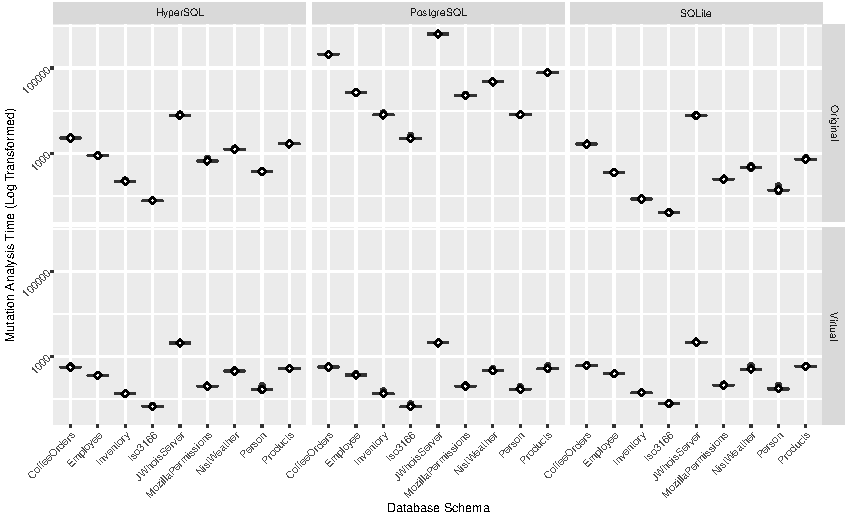
\includegraphics[scale=1.0]{graphics/graphic_bwplot_schema_analysistime_org_vm.pdf}
  \caption{Box plot of the execution time for the standard and virtual mutation analysis techniques.}
  \label{fig:graphic_bwplot_schema_analysistime_org_vm}

  % Details about the box plot from the R documentation:

  % The lower and upper "hinges" correspond to the first and third quartiles (the 25th and 75th percentiles). This differs
  % slightly from the method used by the boxplot function, and may be apparent with small samples. See boxplot.stats for for
  % more information on how hinge positions are calculated for boxplot.

  % The upper whisker extends from the hinge to the highest value that is within 1.5 * IQR of the hinge, where IQR is the
  % inter-quartile range, or distance between the first and third quartiles. The lower whisker extends from the hinge to
  % the lowest value within 1.5 * IQR of the hinge. Data beyond the end of the whiskers are outliers and plotted as points
  % (as specified by Tukey).

  {\small \justifying{ \noindent For a detailed description of the meaning of the boxes in this plot, please refer to
      Section~\ref{sec:experimental-setup}. The boxes in this plot are noticeably compressed because there is little variability in
      the timings across the different configurations.  Since the results from running the standard method on the
      \Postgres~DBMS differ substantially from those with the other techniques and databases, all of the
      data values were log-transformed, thereby best revealing the relevant trends.} \par}

  \vspace*{-1em}

\end{figure*}


Once predicates have been obtained for all integrity constraints pertaining to a database table\footnote{{\scriptsize See McMinn \etal~\cite{McMinn2015} for a full list of functions for the integrity constraints for each of the database management systems that we study in this paper.}}, an {\it acceptance predicate} can be formed. An acceptance predicate describes whether a row of data (such as that which forms part of an \INSERT statement in a test case) conforms to all of the integrity constraints defined on a table, and as such, whether that row of data will be admitted into the database. An acceptance predicate is formed by the conjunction of each of the individual integrity constraint predicates.

% further examples ?

\inlineheading{Performing \VMA} Once acceptance predicates have been obtained for each of the tables of a database schema, they can be used to perform virtual mutation analysis. Instead of submitting the rows of data in the \INSERT statements of a test case directly to the DBMS, rows of data can instead be evaluated by the acceptance predicate relevant to the table that is the subject of the \INSERT. Whereas with standard mutation analysis, we seek to observe a difference in the acceptance and rejection behavior of the DBMS with respect to the \INSERT statements submitted as part of each test case, with \vma we instead seek to monitor difference in truth values of acceptance predicates when evaluated with the data contained within each of the original \INSERT statements of the test suite. Any difference in truth value of an acceptance predicate with the original schema and a mutant indicates that the mutant has been killed.  As with standard mutation analysis, the virtual method can compute a mutation score.

%% PSM - no need to explain this again -- it's introduced in the background
%; that is, the number of mutants killed divided by all mutants under consideration.

Virtual mutation analysis therefore avoids the need to communicate with an actual instance of a DBMS that hosts each of the mutant databases. This saves the cost of setting up the tables of each database according to either the original schema or each of the mutants (through SQL \sql{CREATE TABLE} statements), executing the \INSERT statements in the test suite against the database, and then, finally, restoring the state of the DBMS by removing the database tables (through SQL \sql{DROP TABLE} statements).

One disadvantage of \vma is that a model of the operation of the integrity constraints is needed for the DBMS with which
we wish to test schemas and perform mutation analysis. While integrity constraints tend to operate in broadly the same
way across most DBMSs there is the potential for subtle variations due to differing interpretations of the SQL standard
(as shown with the primary key example with \SQLite). So, while we have a model --- that is accurate for \HyperSQL,
\Postgres and \SQLite and used in this paper --- new models may be required for \mbox{other DBMSs}.


